\documentclass[12pt,twoside]{article}   
\usepackage{light}

\newcommand{\hint}[1]{({\it Hint: #1})}
\newcommand{\card}[1]{\left|#1\right|}
\newcommand{\union}{\cup}
\newcommand{\lgunion}{\bigcup}
\newcommand{\intersect}{\cap}
\newcommand{\lgintersect}{\bigcap}
\newcommand{\cross}{\times}

\hidesolutions
%\showsolutions

\newlength{\strutheight}
\newcommand{\prob}[1]{\mathop{\textup{Pr}} \nolimits \left( #1 \right)}
\newcommand{\prsub}[2]{\mathop{\textup{Pr}_{#1}}\nolimits\left(#2\right)}
\newcommand{\prcond}[2]{%
  \ifinner \settoheight{\strutheight}{$#1 #2$}
  \else    \settoheight{\strutheight}{$\displaystyle#1 #2$} \fi%
  \mathop{\textup{Pr}}\nolimits\left(
    #1\,\left|\protect\rule{0cm}{\strutheight}\right.\,#2
  \right)}
\newcommand{\comment}[1]{}
\newcommand{\cE}{\mathcal{E}}
\renewcommand{\setminus}{-}
\renewcommand{\complement}[1]{\overline{#1}}


\begin{document}
\problemset{10}{November 12, 2008}{Tuesday, November 18}

\begin{problem}{15}
We're interested in the probability that a randomly chosen poker hand (5
cards from a standard 52-card deck) contains cards from at most two suits.

\bparts

\ppart{5} What is an appropriate sample space to use for this problem?  What
are the outcomes in the event, $\cE$, we are interested in?  What are the
probabilities of the individual outcomes in this sample space?

\solution{The natural sample space to use consists of the $\binom{52}{5}$ possible poker hands. We define $\cE$ to be the subset of outcomes in which the 5 cards on the outcome come from at most two suits. The sample space is \emph{uniform}: Each hand is equally likely and comes up with probability $1 / \binom{52}{5}$.}

\ppart{10}  What is $\prob{\cE}$?

\solution{Since the sample space is uniform,
\[
\prob{\cE} = \frac{\card{\cE}}{\dbinom{52}{5}}.
\]
We can count the size of $\cE$ by cases. There are three cases: five cards of the same suit; four cards of one suit and one of another; and three cards of one suit and two of another.

For five of one suit, there are 4 ways to choose the suit and then
$\binom{13}{5}$ ways to choose 5 cards from that suit.

For four of one suit and one of another, there are 4 ways to choose the larger suit and $\binom{13}{4}$ ways to choose 4 cards from that suit. Then there are 3 remaining suits from which to choose 1, and 13 choices for the 1 card of that suit.

Finally, for 3 of one suit and 2 of another, there are 4 ways to choose
the suit of 3 and $\binom{13}{3}$ ways to choose cards for that suit,
and there are 3 remaining suits to choose for the 2 cards, and
$\binom{13}{2}$ choices for the 2 cards of that suit. So the total is
\[
4\cdot \binom{13}{5} + 4 \cdot \binom{13}{4} \cdot 3 \cdot 13 + 4 \cdot
\binom{13}{3} \cdot 3 \cdot \binom{13}{2},
\]
and the probability of at most two suits 
is
\[
\frac{4\cdot \dbinom{13}{5} + 4 \cdot \dbinom{13}{4} \cdot 3 \cdot 13 + 4 \cdot
\dbinom{13}{3} \cdot 3 \cdot \dbinom{13}{2}}{\dbinom{52}{5}}
 = 88/595 \approx 0.15.
\]
}
\eparts

\end{problem}

%%%%%%%%%%%%%%%%%%%%%%%%%%%%%%%%%%%%%%%%%%%%%%%%%%%%%%%%%%%%%%%%%%%%%%%%%%%%%%

\begin{problem}{20} \label{Identities}
Prove the following probabilistic identity, referred to as the {\bf Union Bound}.  You may assume the theorem that the probability of a union of \emph{disjoint} sets is the sum of their probabilities.

\begin{theorem*}
Let $A_1, \dots, A_n$ be a collection of events on some sample space.  Then
\[
\prob{A_1 \union A_2 \union \cdots \union A_n} \leq \sum_{i=1}^n
\prob{A_i}.
\]
\end{theorem*}

\hint{Induction}

\solution{
For all $n \geq 1$, let $P(n)$ be the proposition that the claim is true.

\textit{Base case:} Trivially $\prob{A_1} \leq \prob{A_1}$, so $P(1)$ is true.

\textit{Induction step:} Assume that $P(n)$ is true and show $P(n+1)$ for
$n \geq 1$.
\begin{align*}
\prob{ A_1 \union A_2 \union \cdots \union A_{n+1}} 
 &= \prob{(A_1 \union A_2 \union \cdots \union A_{n}) \union A_{n+1}} \\
 &= \prob{A_1 \union A_2 \union \cdots \union A_{n}} + \prob{A_{n+1}} \\
 &\quad - \prob{(A_1 \union A_2 \union \cdots \union A_{n}) \intersect A_{n+1}}
 &\text{(by~Inclusion-Exclusion)}\\
 &\leq \prob{A_1 \union A_2 \union \cdots \union A_{n}} + \prob{A_{n+1}}\\
 &\leq \sum_{i=1}^{n} \prob{A_{i}} + \prob{A_{n+1}} &\text{(by Ind. Hyp.)} \\
 &= \sum_{i=1}^{n+1} \prob{A_{i}} 
\end{align*}
Thus $P(n)$ is true and the result follows by induction.
}
\end{problem}

%%%%%%%%%%%%%%%%%%%%%%%%%%%%%%%%%%%%%%%%%%%%%%%%%%%%%%%%%%%%%%%%%%%%%%%%%%%%%
%%% Fall07 ps10 problem 1

\begin{problem}{20}
You are organizing a neighborhood census and instruct your census takers
to knock on doors and note the sex of any child that answers the knock.
Assume that there are two children in a household and that girls and boys
are equally likely to be children and to open the door.

A sample space for this experiment has outcomes that are triples whose
first element is either \texttt{B} or \texttt{G} for the sex of the elder
child, likewise for the second element and the sex of the younger child,
and whose third coordinate is \texttt{E} or \texttt{Y} indicating whether
the \emph{e}lder child or \emph{y}ounger child opened the door.  For
example, $(\mathtt{B},\mathtt{G},\mathtt{Y})$ is the outcome that the elder
child is a boy, the younger child is a girl, and the girl opened the door.

\bparts

\ppart{5} Let \emph{T} be the event that the household has two girls,
and \emph{O} be the event that a girl opened the door.  List the outcomes
in \emph{T} and \emph{O}.

\solution{$T=\set{GGE,GGY}, O=\set{GGE,GGY,GBE,BGY}$}

\ppart{5} What is the probability $\prcond{T}{O}$, that both children are
girls, given that a girl opened the door?
\solution{1/2}

\ppart{10} Where is the mistake in the following argument for computing $\prcond{T}{O}$?

\begin{quote}
If a girl opens the door, then we know that there is at least one girl in
the household.  The probability that there is at least one girl is
\[
1 - \prob{\text{both children are boys}} = 1 - (1/2 \times 1/2) = 3/4.
\]
So,
\begin{eqnarray*}
\lefteqn{\prcond{T}{\text{there is at least one girl in the household}}}\\
& = & \frac{\prob{T \intersect \text{there is at least one girl in the household}}}
{\pr{\text{there is at least one girl in the household}}}\\
& = & \frac{\prob{T}}{\pr{\text{there is at least one girl in the household}}}\\
& = & (1/4) / (3/4) = 1/3.
\end{eqnarray*}
Therefore, given that a girl opened the door, the probability that there
are two girls in the household is \textup{1/3}.
\end{quote}

\solution{The argument is a correct proof that 
\[
\prcond{T}{\text{there is at least one girl in the household}} = 1/3.
\]
The problem is that the event, $H$, that the household has at least one girl,
namely,
\[
H = \set{\mathtt{GGE,GGY,GBE,GBY,BGE,BGY}},
\]
is not equal to the event, \emph{O}, that a girl opens the door.  These
two events differ:
\[
H-O = \set{\mathtt{BGE,GBY}},
\]
and their probabilities are different.  So the fallacy is in the final
conclusion where the value of $\prcond{T}{H}$ is taken to be the same as
the value $\prcond{T}{O}$.  Actually, $\prcond{T}{O} = 1/2$.  }

\eparts
\end{problem}

%%%%%%%%%%%%%%%%%%%%%%%%%%%%%%%%%%%%%%%%%%%%%%%%%%%%%%%%%%%%%%%%%%%%%%%%%%%%%%
%
%\begin{problem}{20} \textit{Finalphobia} is a rare
%disease in which the victim has the delusion that he or she is being
%subjected to an intense mathematical examination.
%%
%\begin{itemize}
%\item A person selected uniformly at random has finalphobia with probability
%$1/100$.
%\item A person with finalphobia has shaky hands with probability $9/10$.
%\item A person without finalphobia has shaky hands with probability $1/20$.
%\end{itemize}
%%
%What is the probablility that a person selected uniformly at random
%has finalphobia, given that he or she has shaky hands?
%
%\solution{
%Let $F$ be the event that the randomly-selected person has
%finalphobia, and let $S$ be the event that he or she has shaky hands.
%A tree diagram is worked out below:
%%
%\begin{center}
%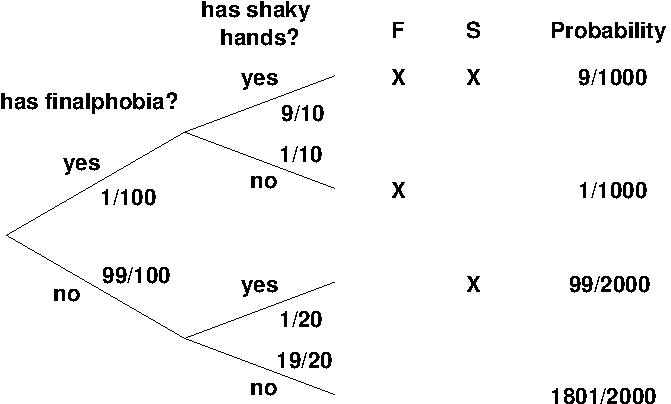
\includegraphics{finalphobia}
%\end{center}
%%
%The probability that a person has finalphobia, given that he or she
%has shaky hands is:
%%
%\begin{align*}
%\prcond{F}{S}
%    & = \frac{\pr{F \cap S}}{\pr{S}} \\
%        & = \frac{9/1000}{9/1000 + 99/2000} \\
%	    & = \frac{18}{18+99} \\
%	        & = \frac{18}{117}
%\end{align*}
%
%So, while it's true that someone with shaky hands is five times more likely to have finalphobia than someone with steady hands, it remains a poor bet---about 1 in 5---that someone with shaky hands actually has does have finalphobia.}
%
%\end{problem}



%%%%%%%%%%%%%%%%%%%%%%%%%%%%%%%%%%%%%%%%%%%%%%%%%%%%%%%%%%%%%%%%%%%%%%%%%%%%%
%%% Fall07 ps10 problem 3

\begin{problem}{25}
Let's play a game!  We repeatedly flip a fair coin.  You have the
sequence $HHT$, and I have the sequence $HTT$.  If your sequence comes
up first, then you win.  If my sequence comes up first, then I win.
For example, if the sequence of tosses is:
\[
TTHTHT\underline{HHT}
\]
then you win.  What is the probability that you win?  It may come as a
surprise that the answer is very different from 1/2.

This problem is tricky, because the game could go on for an arbitrarily
long time.  Draw enough of the tree diagram to see a pattern, and then sum
up the probabilities of the (infinitely many) outcomes in which you win.

It turns out that for any sequence of three flips, there is another
sequence that is likely to come up before it.  So there is no sequence
which turns up earliest! \dots and given any sequence, knowing how to pick
another sequence that comes up sooner more than half the time gives you a
nice chance to fool people gambling at a bar :-)


\solution{A partial tree diagram is shown below.  All edge
probabilities are $1/2$.

\bigskip
\centerline{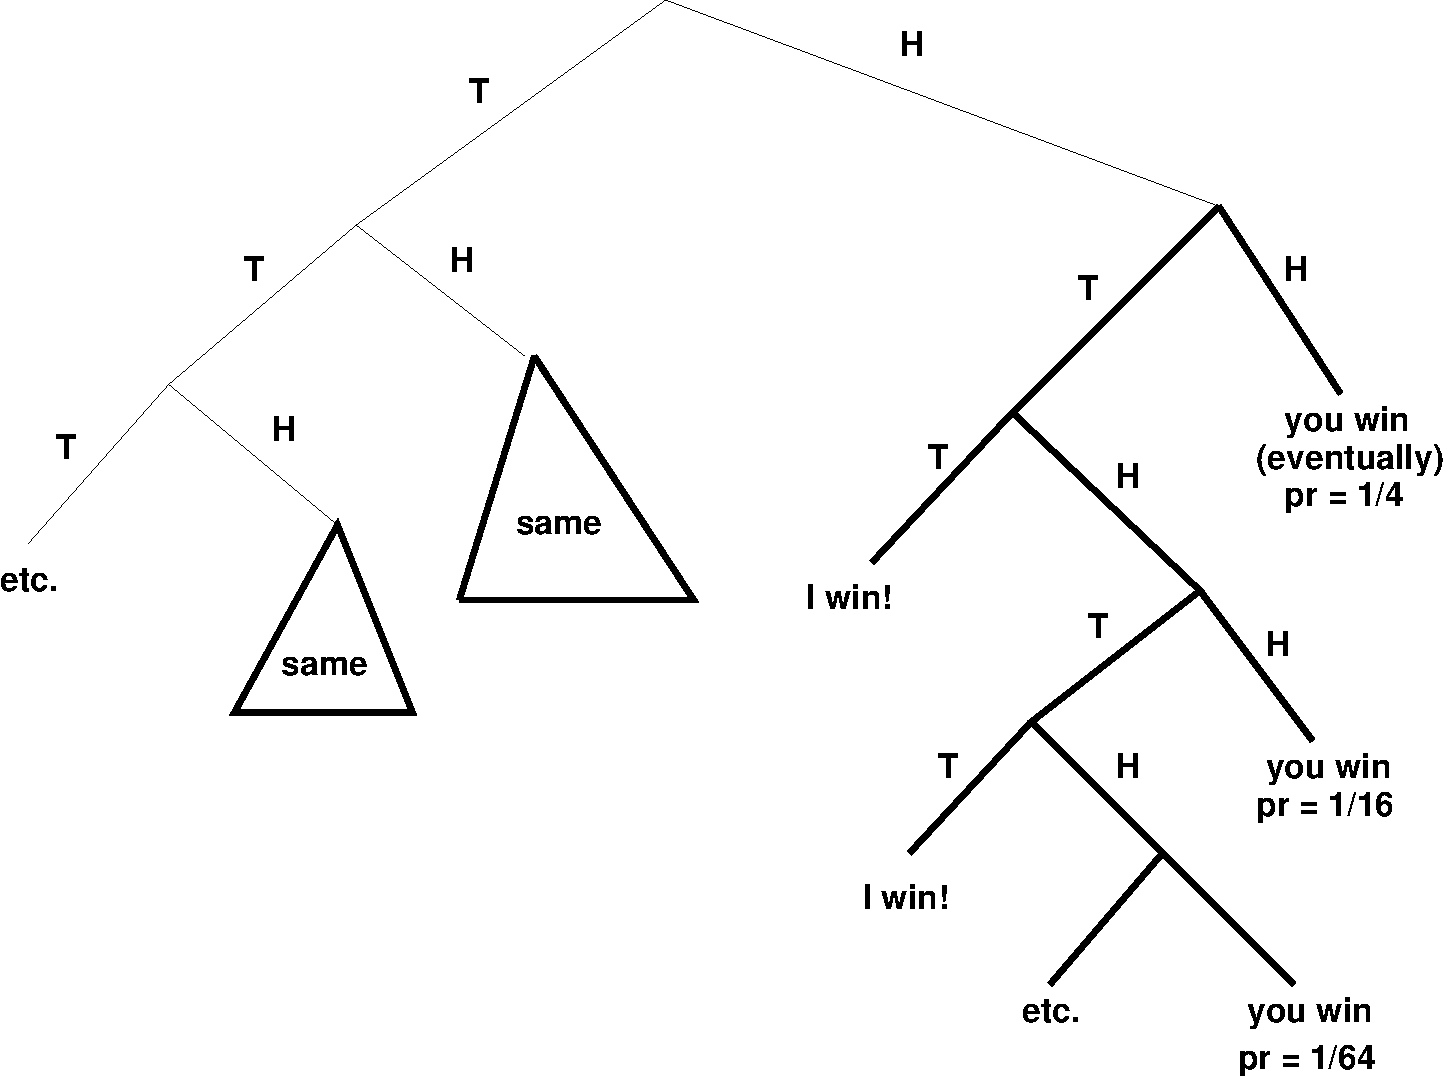
\includegraphics[height=3in]{ps9-HHTtree}}
\bigskip

Let's first focus on the subtree shown in bold.  Note that if two
heads are flipped in a row, then you are guaranteed to win eventually.
The sum of the probabilities of all your winning outcomes in this
subtree is:

\begin{eqnarray*}
\frac{1}{4} + \frac{1}{16} + \frac{1}{64} + \ldots
	& = & \frac{1}{4} \cdot \frac{1}{1 - 1/4} \\
	& = & \frac{1}{3}
\end{eqnarray*}

The uppermost subtree marked {\bf same} is identical to the one
shown in bold, except that each outcome probability is reduced by
$1/2$, because it is one edge farther from the root.  Thus, the sum of
your winning outcomes in this subtree is $1/6$.  Similarly, the sum of
your winning outcomes in the next subtree marked {\bf same} is $1/12$,
and so forth.  Overall, your probability of winning is:

\begin{eqnarray*}
\frac{1}{3} + \frac{1}{6} + \frac{1}{12} + \ldots
	& = & \frac{1}{3} \cdot \frac{1}{1 - 1/2} \\
	& = & \frac{2}{3}
\end{eqnarray*}
}

\end{problem}

%%%%%%%%%%%%%%%%%%%%%%%%%%%%%%%%%
%%% Fall05 ps9 problem 1

\begin{problem}{20}
Professor Plum, Mr. Green, and Miss Scarlet are all plotting to shoot
Colonel Mustard.  If one of these three has both an
\textit{opportunity} and the \textit{revolver}, then that person shoots
Colonel Mustard.  Otherwise, Colonel Mustard escapes.  Exactly one of
the three has an \textit{opportunity} with the following
probabilities:
%
\begin{align*}
\pr{\text{Plum has opportunity}} & = 1 / 6 \\
\pr{\text{Green has opportunity}} & = 2 / 6 \\
\pr{\text{Scarlet has opportunity}} & = 3 / 6
\end{align*}
%
Exactly one has the \textit{revolver} with the following
probabilities, regardless of who has an opportuntity:
%
\begin{align*}
\pr{\text{Plum has revolver}} & = 4 / 8 \\
\pr{\text{Green has revolver}} & = 3 / 8 \\
\pr{\text{Scarlet has revolver}} & = 1 / 8
\end{align*}

\bparts

\ppart{5} Draw a tree diagram for this problem.  Indicate edge and
outcome probabilities.

\solution{
\begin{center}
\begin{picture}(120,270)(0,-30)
\put(0,120){\line(2,3){60}}
\put(0,120){\line(1,0){60}}
\put(0,120){\line(2,-3){60}}
\put(60,30){\line(2,-1){60}}
\put(60,30){\line(1,0){60}}
\put(60,30){\line(2,1){60}}
\put(60,120){\line(2,-1){60}}
\put(60,120){\line(1,0){60}}
\put(60,120){\line(2,1){60}}
\put(60,210){\line(2,-1){60}}
\put(60,210){\line(1,0){60}}
\put(60,210){\line(2,1){60}}
\put(30,180){\makebox(0,0){P}}
\put(30,130){\makebox(0,0){G}}
\put(30,60){\makebox(0,0){S}}
\put(110,245){\makebox(0,0){P}}
\put(110,220){\makebox(0,0){G}}
\put(110,175){\makebox(0,0){S}}
\put(110,155){\makebox(0,0){P}}
\put(110,130){\makebox(0,0){G}}
\put(110,85){\makebox(0,0){S}}
\put(110,65){\makebox(0,0){P}}
\put(110,40){\makebox(0,0){G}}
\put(110,-5){\makebox(0,0){S}}
\put(45,160){\makebox(0,0){$1/6$}}
\put(30,110){\makebox(0,0){$2/6$}}
\put(45,80){\makebox(0,0){$3/6$}}
\put(85,235){\makebox(0,0){$4/8$}}
\put(110,200){\makebox(0,0){$3/8$}}
\put(85,185){\makebox(0,0){$1/8$}}
\put(85,145){\makebox(0,0){$4/8$}}
\put(110,110){\makebox(0,0){$3/8$}}
\put(85,95){\makebox(0,0){$1/8$}}
\put(85,55){\makebox(0,0){$4/8$}}
\put(110,20){\makebox(0,0){$3/8$}}
\put(85,5){\makebox(0,0){$1/8$}}
\put(30,15){\makebox(0,0){\text{opportunity}}}
\put(90,-20){\makebox(0,0){\text{revolver}}}
\put(150,-20){\makebox(0,0){\text{prob.}}}
\put(150,240){\makebox(0,0){$4/48$}}
\put(150,210){\makebox(0,0){$3/48$}}
\put(150,180){\makebox(0,0){$1/48$}}
\put(150,150){\makebox(0,0){$8/48$}}
\put(150,120){\makebox(0,0){$6/48$}}
\put(150,90){\makebox(0,0){$2/48$}}
\put(150,60){\makebox(0,0){$12/48$}}
\put(150,30){\makebox(0,0){$9/48$}}
\put(150,0){\makebox(0,0){$3/48$}}
\end{picture}
\end{center}
}

\ppart{5} What is the probability that Colonel Mustard is shot?

\solution{Denote each outcome with a pair indicating who has the
opportunity and who has the revolver.  In this notation, the event
that Colonel Mustard is shot consists of all outcomes where a single
person has both:
%
\[
\set{(P,P),(G,G),(S,S)}
\]
%
The probability of this event is the sum of the outcome probabilities:
%
\begin{align*}
\pr{\set{(P,P),(G,G),(S,S)}}
    & = \pr{(P,P)} + \pr{(G,G)} + \pr{(S,S)} \\
    & = 4/48 + 6/48 + 3/48 \\
    & = 13/48
\end{align*}
}

\ppart{5} What is the probability that Colonel Mustard is shot, given
that Miss Scarlet does not have the revolver?

\solution{Let $S$ be the event that Colonel Mustard is shot, and let
$N$ be the event that Miss Scarlet does \textit{not} have the
revolver.  The solution is:
%
\begin{align*}
\prcond{S}{N}
    & = \frac{\pr{S \cap N}}{\pr{N}} \\
    & = \frac{\pr{(P,P),(G,G)}}{\pr{(P,P),(P,G),(G,P),(G,G),(S,P),(S,G)}} \\
    & = \frac{\frac{4}{48}+\frac{6}{48}}
             {\frac{4}{48}+\frac{3}{48}+\frac{8}{48}+
              \frac{6}{48}+\frac{12}{48}+\frac{9}{48}} \\
    & = \frac{5}{21}
\end{align*}
}

\ppart{5} What is the probability that Mr. Green had an opportunity,
given that Colonel Mustard was shot?

\solution{Let $G$ be the event that Mr. Green has an opportunity, and
again let $S$ be the event that Colonel Mustard is shot.  Then the
solution is:
%
\begin{align*}
\prcond{G}{S}
    & = \frac{\pr{G \cap S}}{\pr{S}} \\
    & = \frac{\pr{(G,G)}}{\pr{(P,P),(G,G),(S,S)}} \\
    & = \frac{\frac{6}{48}}
             {\frac{4}{48}+\frac{6}{48}+\frac{3}{48}} \\
    & = \frac{6}{13}
\end{align*}
}

\eparts

\end{problem}
\end{document}